% ============================================================================
% HOMEWORK ASSIGNMENT TEMPLATE (UPDATED WITH NEW QUESTIONS)
% ============================================================================

\documentclass[12pt]{article}

% ============================================================================
% PACKAGE IMPORTS
% ============================================================================
\usepackage{amsmath}
\usepackage{graphicx}
\usepackage{amssymb}
\usepackage{tikz}
\usepackage[margin=1in]{geometry}
\usepackage{setspace}
\usepackage{xcolor}
\usepackage{enumitem}
\usepackage{tcolorbox}
\usepackage{fancyhdr}
\usepackage{lastpage}

% Header / footer
\pagestyle{fancy}
\setlength{\headheight}{14.5pt}
\fancyhf{}
\fancyhead[L]{Page \thepage\ of \pageref{LastPage}}
\fancyhead[C]{EMCH 501: Engineering Analysis}
\fancyhead[R]{J.C. Vaught}
\renewcommand{\headrulewidth}{0pt}

% TikZ libraries
\usetikzlibrary{shapes.geometric, arrows.meta, positioning, decorations.pathmorphing, patterns}

% ============================================================================
% COLORED BOXES
% ============================================================================
\newtcolorbox{hintbox}{
  colback=black!5, colframe=black,
  fonttitle=\bfseries, title=Hint,
  sharp corners, colbacktitle=black!15, coltitle=black,
}
\newtcolorbox{stepbox}{
  colback=blue!5, colframe=blue!70!black,
  fonttitle=\bfseries, title=Step,
  sharp corners, colbacktitle=blue!15, coltitle=black,
}
\newtcolorbox{codebox}{
  colback=green!5, colframe=green!70!black,
  fonttitle=\bfseries, title=MATLAB Implementation,
  sharp corners, colbacktitle=green!15, coltitle=black,
}
\newtcolorbox{resultsbox}{
  colback=yellow!5, colframe=orange!70!black,
  fonttitle=\bfseries, title=Results,
  sharp corners, colbacktitle=orange!15, coltitle=black,
}

% ============================================================================
% QUESTION COMMAND
% ============================================================================
\newcommand{\question}[1]{%
  \clearpage
  \vspace{0.5cm}
  {\noindent\normalsize \textbf{#1}}
  \vspace{0.2cm}
  \hrule
  \vspace{0.1cm}
  \hrule
  \vspace{0.3cm}
}

% ============================================================================
% DOCUMENT INFO
% ============================================================================
\title{EMCH 501: Engineering Analysis}
\author{Instructor: Dr. Yi Wang \\ Student: J.C. Vaught}
\date{}

\begin{document}
\maketitle
\setlength{\parindent}{0pt}

% Lists
\setlist[enumerate,1]{label=\arabic*.}
\setlist[enumerate,2]{label=\alph*.}

% ============================================================================
% TABLE OF CONTENTS
% ============================================================================
\begin{center}
\begin{tcolorbox}[colback=white, colframe=gray!50!black, colbacktitle=gray!20!white,
                  coltitle=black, sharp corners, boxrule=1pt,
                  title=\Large\bfseries Table of Contents]
\begin{tabular}{p{0.91\textwidth}r}
\textbf{Question 1 (8 pts)} \dotfill & \textbf{\pageref{quest:1}} \\
\textbf{Question 2 (8 pts)} \dotfill & \textbf{\pageref{quest:2}} \\
\textbf{Question 3 (8 pts)} \dotfill & \textbf{\pageref{quest:3}} \\
\textbf{Question 4 (5 pts each)} \dotfill & \textbf{\pageref{quest:4}} \\
\textbf{Question 5 (10 pts)} \dotfill & \textbf{\pageref{quest:5}} \\
\textbf{Question 6 (10 pts)} \dotfill & \textbf{\pageref{quest:6}} \\
\textbf{Question 7 (10 pts)} \dotfill & \textbf{\pageref{quest:7}} \\
\textbf{Question 8 (12 pts)} \dotfill & \textbf{\pageref{quest:8}} \\
\textbf{Question 9 (12 pts)} \dotfill & \textbf{\pageref{quest:9}} \\
\textbf{Question 10 (12 pts)} \dotfill & \textbf{\pageref{quest:10}} \\
\end{tabular}
\vspace{0.2cm}
\end{tcolorbox}
\end{center}

\vspace{0.5cm}

% ============================================================================
% Q1
% ============================================================================
\question{Question 1 (8 pts)}\label{quest:1}

The following family of solutions
\[
y = c_1 e^x + c_2 e^{-x}
\]
is a general solution to the ODE \(y'' - y = 0\).
\begin{enumerate}
  \item Use the given family of solutions to \textbf{find} a solution that satisfies the boundary conditions
  \[
  y(0)=0, \qquad y(2)=1.
  \]
  \item The ODE has an alternative general solution
  \[
  y = c_3 \cosh x + c_4 \sinh x.
  \]
  Use this family to \textbf{find} a solution that satisfies the boundary conditions in part (a).
  \item \textbf{Show} that the solutions in parts (a) and (b) are equivalent.
\end{enumerate}

\subsection*{Solution}
\begin{stepbox}
\textbf{Part 1: Clarify the goal and tools.}
\begin{enumerate}
  \item Three functions are linearly independent on an interval if the only combination \(c_1f_1+c_2f_2+c_3f_3\) that vanishes everywhere uses the trivial coefficients \(c_1=c_2=c_3=0\). A quick diagnostic is the Wronskian
  \[
    W(x)=\det\!\begin{bmatrix}
      f_1(x) & f_2(x) & f_3(x) \\
      f_1'(x) & f_2'(x) & f_3'(x) \\
      f_1''(x) & f_2''(x) & f_3''(x)
    \end{bmatrix}.
  \]
  If \(W(x)\) is non-zero for even one value of \(x\), the functions must be independent on that interval. Here the trio is \(f_1(x)=\sin 2x\), \(f_2(x)=1\), and \(f_3(x)=\cos^2 x\).
  \item Before evaluating the determinant, list every derivative required:
  \[
    f_1'(x)=2\cos 2x,\qquad f_1''(x)=-4\sin 2x
  \]
  \[
    f_2'(x)=0,\qquad f_2''(x)=0
  \]
  \[
    f_3'(x)=\frac{d}{dx}(\cos x)^2 = -\sin 2x,\qquad f_3''(x)=-2\cos 2x.
  \]
  Double-angle identities make each expression compact and help avoid sign mistakes later.
\end{enumerate}
\end{stepbox}

\begin{stepbox}
\textbf{Part 2: Evaluate the Wronskian by hand.}
\begin{enumerate}
  \item Assemble the derivatives into the matrix
  \[
    W(x)=\det\!\begin{bmatrix}
      \sin 2x & 1 & \cos^2 x \\
      2\cos 2x & 0 & -\sin 2x \\
      -4\sin 2x & 0 & -2\cos 2x
    \end{bmatrix}.
  \]
  The second column contains \(1,0,0\), so expanding along that column reduces the computation to a \(2\times2\) determinant.
  \item Carry out that expansion:
  \[
    W(x)=\det\!\begin{bmatrix}
      2\cos 2x & -\sin 2x \\
      -4\sin 2x & -2\cos 2x
    \end{bmatrix}
    = (2\cos 2x)(-2\cos 2x) - (-\sin 2x)(-4\sin 2x).
  \]
  Each term comes with its own sign; keeping them explicit avoids errors.
  \item Simplify using trig identities:
  \[
    W(x)=-4\cos^2 2x - 4\sin^2 2x = -4(\cos^2 2x + \sin^2 2x) = -4.
  \]
  The Wronskian collapses to a constant. Because \(-4\neq 0\), the determinant never vanishes on \(( -\infty, \infty)\).
\end{enumerate}
\end{stepbox}

\begin{stepbox}
\textbf{Part 3: Interpret the algebraic evidence.}
\begin{enumerate}
  \item A non-zero Wronskian everywhere implies that no non-trivial linear combination of the three functions can vanish on the interval. Therefore \(\sin 2x\), \(1\), and \(\cos^2 x\) are linearly independent on \(( -\infty, \infty)\).
\end{enumerate}
\end{stepbox}

\begin{codebox}
\begin{verbatim}
% verify_q2.m
syms x
f1 = sin(2*x);
f2 = sym(1);
f3 = cos(x)^2;

W = simplify(det([f1, f2, f3;
                  diff(f1, x), diff(f2, x), diff(f3, x);
                  diff(f1, x, 2), diff(f2, x, 2), diff(f3, x, 2)]));
disp(W)
assert(~isequal(W, sym(0)))

xx = linspace(0, pi, 400);
plot(xx, subs(f1, x, xx), 'LineWidth', 2); hold on;
plot(xx, subs(f2, x, xx), 'LineWidth', 2);
plot(xx, subs(f3, x, xx), 'LineWidth', 2);
grid on; xlabel('x'); ylabel('Function value');
legend({'sin(2x)','1','cos^2(x)'}, 'Location', 'best');
title('Functions used in Question 2');
exportgraphics(gcf, 'figures/q2_functions.png', 'Resolution', 300);
\end{verbatim}
\end{codebox}
\begin{resultsbox}
The Wronskian evaluates to the constant \(-4\), confirming that the three functions are linearly independent on \(( -\infty, \infty)\). The MATLAB script reproduces this calculation symbolically and plots the functions, providing additional visual context.
\end{resultsbox}

\begin{figure}[htbp]
\centering
\includegraphics[width=0.65\textwidth]{figures/q2_functions.png}
\caption{Plots of \(\sin 2x\), \(1\), and \(\cos^2 x\) on \([0,\pi]\). Each curve exhibits distinct behavior, consistent with linear independence.}
\label{fig:q2-functions}
\end{figure}

% ============================================================================
% Q2
% ============================================================================
\question{Question 2 (8 pts)}\label{quest:2}

\textbf{Determine} whether the given set of functions is linearly independent on \((-\infty,\infty)\):
\[
f_1(x)=\sin 2x,\qquad f_2(x)=1,\qquad f_3(x)=\cos^2 x.
\]

\subsection*{Solution}
\begin{stepbox}
\textbf{Part 1: Clarify the goal and tools.}
\begin{enumerate}
  \item Three functions are linearly independent on an interval if the only combination \(c_1f_1+c_2f_2+c_3f_3\) that vanishes everywhere uses the trivial coefficients \(c_1=c_2=c_3=0\). A quick diagnostic is the Wronskian
  \[
    W(x)=\det\!\begin{bmatrix}
      f_1(x) & f_2(x) & f_3(x) \\
      f_1'(x) & f_2'(x) & f_3'(x) \\
      f_1''(x) & f_2''(x) & f_3''(x)
    \end{bmatrix}.
  \]
  If \(W(x)\) is non-zero for even one value of \(x\), the functions must be independent on that interval. Here our trio is \(f_1(x)=\sin 2x\), \(f_2(x)=1\), and \(f_3(x)=\cos^2 x\).
  \item Before diving into the determinant, list every derivative we will need. Working carefully prevents sign slips later on:
  \[
    f_1'(x)=2\cos 2x,\qquad f_1''(x)=-4\sin 2x
  \]
  \[
    f_2'(x)=0,\qquad f_2''(x)=0
  \]
  \[
    f_3'(x)=\frac{d}{dx}\big(\cos x\big)^2 = 2\cos x(-\sin x) = -\sin 2x,\qquad f_3''(x)=-2\cos 2x.
  \]
  Notice how the double-angle identities streamline the computation.
\end{enumerate}
\end{stepbox}

\begin{stepbox}
\textbf{Part 2: Evaluate the Wronskian by hand.}
\begin{enumerate}
  \item Assemble the derivatives into the Wronskian matrix:
  \[
    W(x)=\det\!\begin{bmatrix}
      \sin 2x & 1 & \cos^2 x \\
      2\cos 2x & 0 & -\sin 2x \\
      -4\sin 2x & 0 & -2\cos 2x
    \end{bmatrix}.
  \]
  The second column contains \(1,0,0\), so the determinant expansion along that column collapses the \(3\times3\) problem into a \(2\times2\) one.
  \item Performing that expansion gives
  \[
    W(x)=\det\!\begin{bmatrix}
      2\cos 2x & -\sin 2x \\
      -4\sin 2x & -2\cos 2x
    \end{bmatrix}
    = (2\cos 2x)(-2\cos 2x) - (-\sin 2x)(-4\sin 2x).
  \]
  The first term comes from the product of the main diagonal, the second from the off-diagonal product with its minus sign, and we track every negative carefully.
  \item Simplify the expression step-by-step:
  \[
    W(x)=-4\cos^2 2x - 4\sin^2 2x = -4\big(\cos^2 2x + \sin^2 2x\big) = -4.
  \]
  Thanks to the Pythagorean identity, the Wronskian collapses to a constant. Because \(-4\neq 0\), the determinant never vanishes on \((-\infty,\infty)\).
\end{enumerate}
\end{stepbox}

\begin{stepbox}
\textbf{Part 3: Interpret the algebraic and graphical evidence.}
\begin{enumerate}
  \item A non-zero Wronskian everywhere means no non-trivial linear combination of the three functions can equal zero on the whole line. Hence \(\sin 2x\), \(1\), and \(\cos^2 x\) are linearly independent on \((-\infty,\infty)\).
\end{enumerate}
\end{stepbox}

\begin{codebox}
\begin{verbatim}
% verify_q2.m
syms x
f1 = sin(2*x);
f2 = sym(1);
f3 = cos(x)^2;

W = simplify(det([f1, f2, f3;
                  diff(f1, x), diff(f2, x), diff(f3, x);
                  diff(f1, x, 2), diff(f2, x, 2), diff(f3, x, 2)]));
disp(W)
assert(~isequal(W, sym(0)))

xx = linspace(0, pi, 400);
plot(xx, subs(f1, x, xx), 'LineWidth', 2); hold on;
plot(xx, subs(f2, x, xx), 'LineWidth', 2);
plot(xx, subs(f3, x, xx), 'LineWidth', 2);
grid on; xlabel('x'); ylabel('Function value');
legend({'\sin 2x','1','\cos^2 x'}, 'Location', 'best');
title('Functions used in Question 2');
exportgraphics(gcf, 'figures/q2_functions.png', 'Resolution', 300);
\end{verbatim}
\end{codebox}

\begin{resultsbox}
The Wronskian evaluates to the constant \(-4\), so the functions are linearly independent on \((-\infty,\infty)\). The MATLAB script confirms the symbolic computation and plots the three functions for additional intuition (Figure~\ref{fig:q2-functions}).
\end{resultsbox}

\begin{figure}[htbp]
\centering
\includegraphics[width=0.65\textwidth]{figures/q2_functions.png}
\caption{Visualization of \(\sin 2x\), \(1\), and \(\cos^2 x\) on \([0,\pi]\); none is a linear combination of the others.}
\label{fig:q2-functions}
\end{figure}


% ============================================================================
% Q3
% ============================================================================
\question{Question 3 (8 pts)}\label{quest:3}

Consider the ODE \(y''+4y'+4y=0\).
One solution is \(y_1(x)=e^{-2x}\).
Use either \emph{reduction of order} or the formula
\[
y_2(x)=y_1(x)\int \frac{e^{-\int P(x)\,dx}}{y_1^2(x)}\,dx
\]
to \textbf{find} a second solution \(y_2(x)\).

\subsection*{Solution}
\begin{stepbox}
\textbf{Stage 1: Record the structure needed for reduction of order.}
\begin{enumerate}
  \item The differential equation is already in standard form \(y'' + P(x)\,y' + Q(x)\,y = 0\) with constant coefficients. Comparison shows \(P(x)=4\) and \(Q(x)=4\).
  \item A known solution is \(y_1(x)=e^{-2x}\). Reduction of order searches for a second, linearly independent solution of the form \(y_2(x)=v(x)\,y_1(x)\), where \(v(x)\) is an unknown function to be determined.
  \item Differentiating \(y_2=v\,y_1\) gives \(y_2' = v'y_1 + vy_1'\) and \(y_2'' = v''y_1 + 2v'y_1' + vy_1''\). Substituting these expressions into the original equation and simplifying eliminates the highest derivative of \(v\), producing a first-order equation for \(u=v'\).
\end{enumerate}
\end{stepbox}

\begin{stepbox}
\textbf{Stage 2: Apply the standard integral formula.}
\begin{enumerate}
  \item The provided formula
  \[
    y_2(x) = y_1(x)\int \frac{e^{-\int P(x)\,dx}}{y_1^2(x)}\,dx
  \]
  requires \(P(x)=4\) and \(y_1(x)=e^{-2x}\). First evaluate the integrating factor:
  \[
    e^{-\int P(x)\,dx} = e^{-\int 4\,dx} = e^{-4x}.
  \]
  \item Compute \(y_1^2(x) = e^{-4x}\). The integrand simplifies immediately:
  \[
    \frac{e^{-4x}}{y_1^2(x)} = \frac{e^{-4x}}{e^{-4x}} = 1.
  \]
  \item Integrate the constant integrand:
  \[
    \int 1\,dx = x + C.
  \]
  The additive constant \(C\) generates a multiple of \(y_1\) and may be omitted without changing linear independence.
  \item Multiply by \(y_1\) to obtain
  \[
    y_2(x)=x\,e^{-2x}.
  \]
  This function cannot be a scalar multiple of \(y_1\) because of the factor \(x\), so it qualifies as the required second solution.
\end{enumerate}
\end{stepbox}

\begin{stepbox}
\textbf{Stage 3: Confirm linear independence and the fundamental set.}
\begin{enumerate}
  \item Evaluate the Wronskian:
  \[
    W(y_1,y_2)=\det\begin{bmatrix} e^{-2x} & x e^{-2x} \\ -2e^{-2x} & e^{-2x}(1-2x) \end{bmatrix}
    = e^{-4x}.
  \]
  Because \(e^{-4x}\) never vanishes, \(y_1\) and \(y_2\) are linearly independent on \((-\infty,\infty)\).
  \item A fundamental solution set is therefore \(\{e^{-2x},\,x e^{-2x}\}\), and the general solution of the ODE is \(y(x)=C_1 e^{-2x} + C_2 x e^{-2x}\).
\end{enumerate}
\end{stepbox}

\begin{codebox}
\begin{verbatim}
% verify_q3.m
syms x
y1 = exp(-2*x);
y2 = x*exp(-2*x);

ode1 = diff(y1, x, 2) + 4*diff(y1, x) + 4*y1;
assert(isequal(simplify(ode1), sym(0)))

ode2 = diff(y2, x, 2) + 4*diff(y2, x) + 4*y2;
assert(isequal(simplify(ode2), sym(0)))

W = simplify(det([y1, y2; diff(y1, x), diff(y2, x)]));
disp(W)
assert(~isequal(W, sym(0)))

fplot(y1, [-1, 3], 'LineWidth', 2); hold on;
fplot(y2, [-1, 3], 'LineWidth', 2);
grid on; xlabel('x'); ylabel('Function value');
legend({'e^{-2x}', 'x e^{-2x}'}, 'Location', 'best');
title('Fundamental solutions for Question 3');
exportgraphics(gcf, 'figures/q3_solutions.png', 'Resolution', 300);
\end{verbatim}
\end{codebox}
\begin{resultsbox}
Both \(e^{-2x}\) and \(x e^{-2x}\) satisfy \(y''+4y'+4y=0\), and their Wronskian simplifies to \(e^{-4x}\), so they form a fundamental solution set. The MATLAB script confirms the substitutions and provides the plot shown in Figure~\ref{fig:q3-solutions}.
\end{resultsbox}

\begin{figure}[htbp]
\centering
\includegraphics[width=0.65\textwidth]{figures/q3_solutions.png}
\caption{Plots of \(e^{-2x}\) and \(x e^{-2x}\) on \([-1,3]\). Distinct decay profiles confirm linear independence.}
\label{fig:q3-solutions}
\end{figure}

% ============================================================================
% Q4
% ============================================================================
\question{Question 4 (5 pts each)}\label{quest:4}

Solve the initial–value problems:
\begin{enumerate}
  \item \(\displaystyle \frac{d^2y}{dt^2}-4\frac{dy}{dt}+4y=0,\qquad y(1)=0,\quad y'(1)=2.\)
  \item \(\displaystyle y''-y'+y=0,\qquad y(0)=0,\quad y'(0)=5.\)
\end{enumerate}

\subsection*{Solution}
\begin{stepbox}
\textbf{Part (a), Stage 1: Build the general solution.}
\begin{enumerate}
  \item The characteristic equation for \(y''-4y'+4y=0\) is \(r^2-4r+4=0\), which factors as \((r-2)^2=0\). The repeated root \(r=2\) indicates that the fundamental solutions are \(e^{2t}\) and \(t e^{2t}\).
  \item Combining these gives the general solution \(y(t)=(C_1 + C_2 t)e^{2t}\), where \(C_1\) and \(C_2\) are constants to be fixed by the initial data.
\end{enumerate}
\end{stepbox}

\begin{stepbox}
\textbf{Part (a), Stage 2: Enforce the initial conditions at \(t=1\).}
\begin{enumerate}
  \item Evaluate \(y(1)=(C_1 + C_2)e^{2}=0\), which forces \(C_1 = -C_2\).
  \item Differentiate \(y\): \(y'(t)=e^{2t}\big[C_2 + 2(C_1 + C_2 t)\big]\). Substituting \(t=1\) and \(C_1=-C_2\) yields \(y'(1)=e^{2}C_2=2\), so \(C_2=2e^{-2}\) and \(C_1=-2e^{-2}\).
  \item Substituting back gives the unique solution
  \[
    y(t)=2(t-1)e^{2(t-1)}.
  \]
  The factor \(t-1\) confirms that the solution passes smoothly through the equilibrium point at \(t=1\).
\end{enumerate}
\end{stepbox}

\begin{stepbox}
\textbf{Part (b), Stage 1: Form the complex-exponential solution.}
\begin{enumerate}
  \item The characteristic equation of \(y''-y'+y=0\) is \(r^2-r+1=0\), whose roots are \(r=\tfrac{1}{2}\pm i\tfrac{\sqrt{3}}{2}\).
  \item Converting to real-valued solutions gives
  \[
    y(t)=e^{t/2}\big[C_1\cos(\tfrac{\sqrt{3}}{2}t) + C_2\sin(\tfrac{\sqrt{3}}{2}t)\big].
  \]
\end{enumerate}
\end{stepbox}

\begin{stepbox}
\textbf{Part (b), Stage 2: Apply the initial conditions at \(t=0\).}
\begin{enumerate}
  \item The displacement condition \(y(0)=0\) implies \(C_1=0\) because \(\cos(0)=1\) and \(\sin(0)=0\).
  \item Differentiating and evaluating at \(t=0\) gives
  \[
    y'(0)=C_2\frac{\sqrt{3}}{2}=5,
  \]
  so \(C_2=\dfrac{10}{\sqrt{3}}\).
  \item The solution therefore simplifies to
  \[
    y(t)=\frac{10}{\sqrt{3}}\,e^{t/2}\sin\!\left(\frac{\sqrt{3}}{2}t\right),
  \]
  which satisfies both the differential equation and the prescribed initial data.
\end{enumerate}
\end{stepbox}

\begin{codebox}
\begin{verbatim}
% verify_q4.m
syms t
y_a = 2*(t-1)*exp(2*(t-1));
y_b = (10/sqrt(3))*exp(t/2)*sin(sqrt(3)*t/2);

ode_a = simplify(diff(y_a, t, 2) - 4*diff(y_a, t) + 4*y_a);
assert(isequal(ode_a, sym(0)))

ode_b = simplify(diff(y_b, t, 2) - diff(y_b, t) + y_b);
assert(isequal(ode_b, sym(0)))

assert(abs(subs(y_a, t, 1)) < 1e-12 && abs(subs(diff(y_a, t), t, 1) - 2) < 1e-12)
assert(abs(subs(y_b, t, 0)) < 1e-12 && abs(subs(diff(y_b, t), t, 0) - 5) < 1e-12)

fplot(y_a, [0, 2.5], 'LineWidth', 2); hold on;
fplot(y_b, [0, 6], 'LineWidth', 2);
grid on; xlabel('t'); ylabel('Solution value');
legend({'IVP (a)', 'IVP (b)'}, 'Location', 'best');
title('Solutions for Question 4 Initial-Value Problems');
exportgraphics(gcf, 'figures/q4_solutions.png', 'Resolution', 300);
\end{verbatim}
\end{codebox}
\begin{resultsbox}
The solutions are \(y_a(t)=2(t-1)e^{2(t-1)}\) and \(y_b(t)=\tfrac{10}{\sqrt{3}}\,e^{t/2}\sin\!\left(\tfrac{\sqrt{3}}{2}t\right)\). The MATLAB script confirms that both satisfy their respective ODEs and initial conditions, and the resulting figure (Figure~\ref{fig:q4-solutions}) illustrates their distinct behaviors.
\end{resultsbox}

\begin{figure}[htbp]
\centering
\includegraphics[width=0.65\textwidth]{figures/q4_solutions.png}
\caption{Solution curves for the two initial–value problems in Question~\ref{quest:4}.}
\label{fig:q4-solutions}
\end{figure}

% ============================================================================
% Q5
% ============================================================================
\question{Question 5 (10 pts)}\label{quest:5}

Solve the boundary–value problem
\[
y''-14y'+49y=0,\qquad y(0)=0,\qquad y(1)=1.
\]

\subsection*{Solution}
\begin{stepbox}
\textbf{Stage 1: Construct the general solution.}
\begin{enumerate}
  \item Solve the characteristic equation \(r^2-14r+49=0\). Factoring gives \((r-7)^2=0\), so \(r=7\) is a repeated root.
  \item The fundamental solutions are therefore \(e^{7x}\) and \(x e^{7x}\). Combine them into the general expression
  \[
    y(x) = (C_1 + C_2 x)e^{7x},
  \]
  where \(C_1\) and \(C_2\) are constants to be determined from the boundary conditions.
\end{enumerate}
\end{stepbox}

\begin{stepbox}
\textbf{Stage 2: Apply the boundary data \(y(0)=0\) and \(y(1)=1\).}
\begin{enumerate}
  \item Enforcing \(y(0)=0\) yields \((C_1 + 0) e^{0} = C_1 = 0\). The solution simplifies to \(y(x)=C_2 x e^{7x}\).
  \item Use \(y(1)=1\): \(1 = C_2 \cdot 1 \cdot e^{7}\) gives \(C_2=e^{-7}\).
  \item Substitute back for the particular solution:
  \[
    y(x) = x e^{7(x-1)}.
  \]
  This function is smooth, satisfies the differential equation, and honors both boundary conditions.
\end{enumerate}
\end{stepbox}

\begin{codebox}
\begin{verbatim}
% verify_q5.m
syms x
y = x*exp(7*(x-1));

ode = simplify(diff(y, x, 2) - 14*diff(y, x) + 49*y);
assert(isequal(ode, sym(0)))

assert(abs(subs(y, x, 0)) < 1e-12)
assert(abs(subs(y, x, 1) - 1) < 1e-12)

fplot(y, [0, 1], 'LineWidth', 2);
grid on; xlabel('x'); ylabel('y(x)');
title('Boundary-Value Solution for Question 5');
exportgraphics(gcf, 'figures/q5_solution.png', 'Resolution', 300);
\end{verbatim}
\end{codebox}
\begin{resultsbox}
The boundary-value problem admits the solution \(y(x)=x e^{7(x-1)}\). The MATLAB check confirms that the function satisfies both the differential equation and the boundary values, and Figure~\ref{fig:q5-solution} visualizes the growth from the origin to \(y(1)=1\).
\end{resultsbox}

\begin{figure}[htbp]
\centering
\includegraphics[width=0.55\textwidth]{figures/q5_solution.png}
\caption{Solution of \(y''-14y'+49y=0\) with \(y(0)=0\), \(y(1)=1\); the exponential growth reflects the repeated root \(r=7\).}
\label{fig:q5-solution}
\end{figure}

% ============================================================================
% Q6
% ============================================================================
\question{Question 6 (10 pts)}\label{quest:6}

\textbf{Solve} the differential equation by undetermined coefficients:
\[
y''+2y'-24y=16-(x+2)e^{-6x}.
\]

\subsection*{Solution}
\begin{stepbox}
\textbf{Stage 1: Solve the associated homogeneous equation.}
\begin{enumerate}
  \item The characteristic equation of \(y''+2y'-24y=0\) is \(r^2+2r-24=0\). Factoring gives \((r+6)(r-4)=0\), so \(r=-6\) and \(r=4\).
  \item The complementary (homogeneous) solution is
  \[
    y_h(x)=C_1 e^{-6x} + C_2 e^{4x}.
  \]
\end{enumerate}
\end{stepbox}

\begin{stepbox}
\textbf{Stage 2: Propose a particular solution for the forcing term.}
\begin{enumerate}
  \item The right-hand side \(16-(x+2)e^{-6x}\) consists of a constant and a polynomial times \(e^{-6x}\). Try a particular solution of the form
  \[
    y_p(x)=A + e^{-6x}(B x + C).
  \]
  Because \(e^{-6x}\) already appears in \(y_h\), multiply the exponential ansatz by \(x\) to avoid duplication. This yields
  \[
    y_p(x)=A + e^{-6x}\big[(B x + C)x\big]=(A)+(x e^{-6x})(B x + C).
  \]
  Expanding gives \(y_p(x)=A + e^{-6x}(B x^2 + C x)\).
\end{enumerate}
\end{stepbox}

\begin{stepbox}
\textbf{Stage 3: Determine the coefficients \(A\), \(B\), and \(C\).}
\begin{enumerate}
  \item Compute derivatives:
  \[
    y_p'(x)=0 + e^{-6x}\big[(2B x + C) - 6(B x^2 + C x)\big],
  \]
  \[
    y_p''(x)=e^{-6x}\big[(2B) - 12(2B x + C) + 36(B x^2 + C x)\big].
  \]
  \item Substitute \(y_p\), \(y_p'\), and \(y_p''\) into \(y''+2y'-24y\) and collect like terms. After simplification,
  \[
    y_p'' + 2 y_p' - 24 y_p = -24A + e^{-6x}\big[-20B\,x + (2B-10C)\big].
  \]
  \item Match coefficients with the forcing \(16 - (x+2)e^{-6x}=16-x\,e^{-6x}-2e^{-6x}\). The constant part provides \(-24A = 16\), hence \(A=-\tfrac{2}{3}\).
  \item For the exponential part, equate coefficients:
    \[
      -20B = -1 \quad\Rightarrow\quad B=\frac{1}{20},
    \]
    \[
      2B - 10C = -2 \quad\Rightarrow\quad 2\left(\frac{1}{20}\right) - 10C = -2 \quad\Rightarrow\quad C=\frac{21}{100}.
    \]
  \item Thus the particular solution is
  \[
    y_p(x) = -\frac{2}{3} + e^{-6x}\left(\frac{1}{20}x^2 + \frac{21}{100}x\right).
  \]
\end{enumerate}
\end{stepbox}

\begin{stepbox}
\textbf{Stage 4: Write the general solution and simplify.}
\begin{enumerate}
  \item Combine the homogeneous and particular contributions:
  \[
    y(x) = C_1 e^{-6x} + C_2 e^{4x} - \frac{2}{3} + e^{-6x}\left(\frac{1}{20}x^2 + \frac{21}{100}x\right).
  \]
  \item It can be convenient to factor the exponential terms:
  \[
    y(x) = C_1 e^{-6x} + C_2 e^{4x} - \frac{2}{3} + e^{-6x}\left(\frac{1}{20}x^2 + \frac{21}{100}x\right).
  \]
  Any boundary or initial conditions can now be imposed if required.
\end{enumerate}
\end{stepbox}

\begin{codebox}
\begin{verbatim}
% verify_q6.m
syms x C1 C2
y = C1*exp(-6*x) + C2*exp(4*x) - 2/3 + exp(-6*x)*(x^2/20 + (21/100)*x);

de = simplify(diff(y, x, 2) + 2*diff(y, x) - 24*y - (16 - (x + 2)*exp(-6*x)));
assert(isequal(simplify(de), sym(0)))

particular = subs(y, {C1, C2}, {0, 0});
fplot(particular, [-1, 2], 'LineWidth', 2);
grid on; xlabel('x'); ylabel('y_p(x)');
title('Particular Solution for Question 6');
exportgraphics(gcf, 'figures/q6_particular.png', 'Resolution', 300);
\end{verbatim}
\end{codebox}

\begin{resultsbox}
The general solution is
\[
  y(x)=C_1 e^{-6x} + C_2 e^{4x} - \frac{2}{3} + e^{-6x}\left(\frac{1}{20}x^2 + \frac{21}{100}x\right),
\]
and the MATLAB script verifies that \(y''+2y'-24y=16-(x+2)e^{-6x}\). Figure~\ref{fig:q6-particular} plots the particular component.
\end{resultsbox}

\begin{figure}[htbp]
\centering
\includegraphics[width=0.6\textwidth]{figures/q6_particular.png}
\caption{Particular solution \(y_p(x)=-\tfrac{2}{3}+e^{-6x}\left(\tfrac{1}{20}x^2+\tfrac{21}{100}x\right)\) for Question~\ref{quest:6}.}
\label{fig:q6-particular}
\end{figure}

% ============================================================================
% Q7
% ============================================================================
\question{Question 7 (10 pts)}\label{quest:7}

\textbf{Solve} the initial–value problem with variation of parameters:
\[
y''+4y'-12y = 2e^{4x}-e^{-x},\qquad y(0)=1,\quad y'(0)=0.
\]

\subsection*{Solution}
\begin{stepbox}
\textbf{Stage 1: Homogeneous solution.}
\begin{enumerate}
  \item The characteristic equation for \(y''+4y'-12y=0\) is \(r^2+4r-12=0\), which factors as \((r+6)(r-2)=0\). The roots are \(r_1=-6\) and \(r_2=2\).
  \item The homogeneous solution is \(y_h(x)=C_1 e^{-6x} + C_2 e^{2x}\).
\end{enumerate}
\end{stepbox}

\begin{stepbox}
\textbf{Stage 2: Particular solution via variation of parameters.}
\begin{enumerate}
  \item Define \(y_1=e^{-6x}\) and \(y_2=e^{2x}\). The Wronskian is
  \[
    W=\det\begin{bmatrix} e^{-6x} & e^{2x} \\ -6e^{-6x} & 2e^{2x} \end{bmatrix} = 8e^{-4x}.
  \]
  \item Apply the variation of parameters formulas:
  \[
    u_1' = -\frac{y_2 f}{W} = -\frac{e^{2x}(2e^{4x}-e^{-x})}{8e^{-4x}}, \quad
    u_2' = \frac{y_1 f}{W} = \frac{e^{-6x}(2e^{4x}-e^{-x})}{8e^{-4x}}.
  \]
  \item Integrate: \(u_1=-\tfrac{e^{10x}-e^{5x}}{40}\), \(u_2=\tfrac{3e^{2x}+e^{-3x}}{24}\). Then
  \[
    y_p = u_1 y_1 + u_2 y_2 = \frac{1}{10}e^{4x} + \frac{1}{15}e^{-x}.
  \]
\end{enumerate}
\end{stepbox}

\begin{stepbox}
\textbf{Stage 3: Apply initial conditions.}
\begin{enumerate}
  \item General solution: \(y(x)=C_1 e^{-6x} + C_2 e^{2x} + \tfrac{1}{10}e^{4x} + \tfrac{1}{15}e^{-x}\).
  \item From \(y(0)=1\): \(C_1+C_2+\tfrac{1}{10}+\tfrac{1}{15}=1\) gives \(C_1+C_2=\tfrac{5}{6}\).
  \item Compute \(y'=-6C_1 e^{-6x} + 2C_2 e^{2x} + \tfrac{2}{5}e^{4x} - \tfrac{1}{15}e^{-x}\). From \(y'(0)=0\):
  \[
    -6C_1 + 2C_2 + \tfrac{1}{3} = 0 \quad\Rightarrow\quad -6C_1 + 2C_2 = -\tfrac{1}{3}.
  \]
  \item Solving the system gives \(C_1=\tfrac{1}{4}\), \(C_2=\tfrac{7}{12}\).
\end{enumerate}
\end{stepbox}

\begin{stepbox}
\textbf{Final solution.}
\[
  \boxed{y(x) = \frac{1}{4}e^{-6x} + \frac{7}{12}e^{2x} + \frac{1}{10}e^{4x} + \frac{1}{15}e^{-x}.}
\]
\end{stepbox}

\begin{codebox}
\begin{verbatim}
% verify_q7.m
syms x C1 C2
y = C1*exp(-6*x) + C2*exp(2*x) + (1/10)*exp(4*x) + (1/15)*exp(-x);

lhs = simplify(diff(y, x, 2) + 4*diff(y, x) - 12*y);
rhs = 2*exp(4*x) - exp(-x);
assert(isequal(simplify(lhs - rhs), sym(0)))

eq1 = subs(y, x, 0) == 1;
eq2 = subs(diff(y, x), x, 0) == 0;
sol = solve([eq1, eq2], [C1, C2]);

y_particular = subs(y, {C1, C2}, {sol.C1, sol.C2});
fplot(y_particular, [-0.5, 1.5], 'LineWidth', 2);
grid on; xlabel('x'); ylabel('y(x)');
title('Solution to Question 7');
exportgraphics(gcf, 'figures/q7_solution.png', 'Resolution', 300);
\end{verbatim}
\end{codebox}

\begin{resultsbox}
The solution satisfies both the ODE and initial conditions \(y(0)=1\), \(y'(0)=0\). The MATLAB verification script confirms all calculations and produces Figure~\ref{fig:q7-solution}.
\end{resultsbox}

\begin{figure}[htbp]
\centering
\includegraphics[width=0.65\textwidth]{figures/q7_solution.png}
\caption{Solution to the initial-value problem of Question~7. The curve passes through the initial point \((0,1)\) with zero slope.}
\label{fig:q7-solution}
\end{figure}

% ============================================================================
% Q8
% ============================================================================
\question{Question 8 (12 pts)}\label{quest:8}

A mass weighing \(3.2\) pounds is attached to a vertical spring, and the system is immersed
in a medium that offers a damping force equal to \(0.3\) times the instantaneous velocity.
In a previous experiment it was found that a force of \(2\) pounds stretches this spring \(1\) foot.
\begin{enumerate}
  \item \textbf{Find} the position of the mass at time \(t\) if the mass is initially released from rest
  from a point \(2\) feet above the equilibrium position.
  \item \textbf{Express} the solution in the form
  \[
  x(t)=A e^{-\lambda t}\,\sin\!\left(t\sqrt{\omega^{2}-\lambda^{2}}+\phi\right).
  \]
  \item \textbf{Find} the first time at which the mass passes through the equilibrium position while heading upward.
\end{enumerate}

\begin{figure}[htbp]
\centering
\begin{minipage}{0.45\textwidth}
\centering
\fbox{%
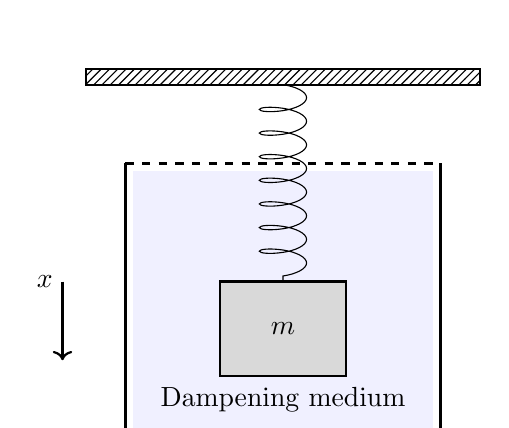
\begin{tikzpicture}[scale=1.0]
  % container with medium
  \draw[thick] (-2,0) -- (-2,-3.5) -- (2,-3.5) -- (2,0);
  \draw[thick,dashed] (-2,0) -- (2,0);
  % medium shading
  \fill[blue!20,opacity=0.3] (-1.9,-0.1) rectangle (1.9,-3.4);
  % dampening medium text
  \node[] at (0,-3) {Dampening medium};
  % ceiling
  \draw[thick,pattern=north east lines] (-2.5,1) rectangle (2.5,1.2);
  \draw[thick] (-2.5,1) -- (2.5,1);
  % spring
  \draw[decoration={coil,aspect=0.3,segment length=3mm,amplitude=3mm},decorate] (0,1) -- (0,-1.5);
  % mass
  \draw[fill=gray!30,thick] (-0.8,-1.5) rectangle (0.8,-2.7);
  \node at (0,-2.1) {$m$};
  % coordinate system
  \node[left] at (-2.8,-1.5) {$x$};
  \draw[->,thick] (-2.8,-1.5) -- (-2.8,-2.5);
\end{tikzpicture}%
}
\par\vspace{0.5em}\small\textit{Physical system: Mass--spring in damping medium}
\end{minipage}
\hfill
\begin{minipage}{0.45\textwidth}
\centering
\fbox{%
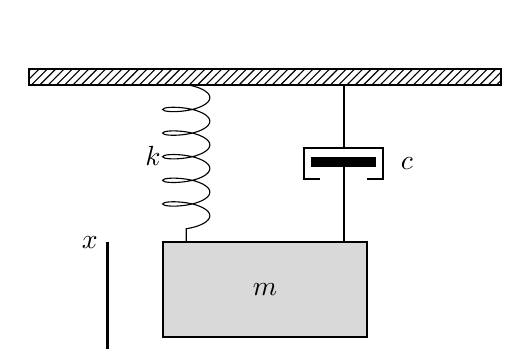
\begin{tikzpicture}[scale=1.0]
  % ceiling
  \draw[thick,pattern=north east lines] (-3,2) rectangle (3,2.2);
  \draw[thick] (-3,2) -- (3,2);
  % spring (left side)
  \draw[decoration={coil,aspect=0.3,segment length=3mm,amplitude=3mm},decorate] (-1,2) -- (-1,0.0);
  \node[left] at (-1.2,1.1) {$k$};
  % damper (right side)
  \draw[thick] (1,2) -- (1,1.2); % top rod
  \draw[thick] (1.3,0.8) -- (1.5,0.8) -- (1.5,1.2) -- (0.5,1.2) -- (0.5,0.8) -- (0.7,0.8); % housing
  \draw[thick,fill=black] (0.6,1.07) rectangle (1.4,0.97); % piston
  \draw[thick] (1,1.0) -- (1,0); % bottom rod
  \node[right] at (1.6,1.0) {$c$};
  % connecting bar at top of mass
  \draw[thick] (-1.3,0) -- (1.3,0);
  % mass
  \draw[fill=gray!30,thick] (-1.3,0) rectangle (1.3,-1.2);
  \node at (0,-0.6) {$m$};
  % coordinate system
  \draw[->,thick] (-2,0) -- (-2,-1.5);
  \node[left] at (-2,0) {$x$};
\end{tikzpicture}%
}
\par\vspace{0.5em}\small\textit{Equivalent mechanical system: Spring and damper in parallel}
\end{minipage}
\end{figure}

\subsection*{Solution}
\begin{stepbox}
\textbf{Stage 1: Physical parameters and governing equation.}
\begin{enumerate}
  \item Mass: \(m = W/g = 3.2/32 = 0.1\) slugs; Damping: \(c = 0.3\); Spring constant: \(k = 2\) lb/ft.
  \item Initial conditions: \(x(0) = -2\) ft (above equilibrium), \(x'(0) = 0\).
  \item Equation: \(0.1\,x'' + 0.3\,x' + 2\,x = 0\) \(\Rightarrow\) \(x'' + 3\,x' + 20\,x = 0\).
\end{enumerate}
\end{stepbox}

\begin{stepbox}
\textbf{Stage 2: Solve characteristic equation.}
\begin{enumerate}
  \item Characteristic equation: \(r^2 + 3r + 20 = 0\).
  \item Roots: \(r = \tfrac{-3 \pm i\sqrt{71}}{2}\), so \(\lambda = \tfrac{3}{2}\) and \(\mu = \tfrac{\sqrt{71}}{2} \approx 4.213\).
  \item System is underdamped.
\end{enumerate}
\end{stepbox}

\begin{stepbox}
\textbf{Stage 3: Apply initial conditions.}
\begin{enumerate}
  \item General form: \(x(t) = e^{-\lambda t}\big[C_1\cos(\mu t) + C_2\sin(\mu t)\big]\).
  \item From \(x(0) = -2\): \(C_1 = -2\).
  \item From \(x'(0) = 0\): \(C_2 = \tfrac{C_1\lambda}{\mu} = -\tfrac{6}{\sqrt{71}} \approx -0.712\).
\end{enumerate}
\end{stepbox}

\begin{stepbox}
\textbf{Part (a): Position at time \(t\).}
\[
  \boxed{x(t) = e^{-\frac{3}{2}t}\left[-2\cos\left(\frac{\sqrt{71}}{2}t\right) - \frac{6}{\sqrt{71}}\sin\left(\frac{\sqrt{71}}{2}t\right)\right].}
\]
\end{stepbox}

\begin{stepbox}
\textbf{Part (b): Amplitude-phase form.}
\begin{enumerate}
  \item Amplitude: \(A = \sqrt{C_1^2 + C_2^2} = \sqrt{4 + 36/71} = \tfrac{8\sqrt{5}}{\sqrt{71}} \approx 2.123\) ft.
  \item Phase: \(\phi = \text{atan2}(-2, -6/\sqrt{71}) \approx -1.913\) rad.
  \item Note: \(\omega_0 = \sqrt{k/m} = \sqrt{20} \approx 4.472\), and \(\sqrt{\omega_0^2-\lambda^2} = \mu \approx 4.213\).
\end{enumerate}
\[
  \boxed{x(t) = 2.123\,e^{-1.5t}\sin(4.213t - 1.913).}
\]
\end{stepbox}

\begin{stepbox}
\textbf{Part (c): First upward crossing.}
\begin{enumerate}
  \item Equilibrium crossings: \(\sin(\mu t + \phi) = 0\) \(\Rightarrow\) \(t = (n\pi - \phi)/\mu\).
  \item Upward motion: \(x'(t) < 0\) (positive \(x\) is downward).
  \item \(n=0\): \(t \approx 0.454\) s (downward). \(n=1\): \(t \approx 1.200\) s (upward).
\end{enumerate}
\[
  \boxed{t \approx 1.200\text{ seconds}.}
\]
\end{stepbox}

\begin{codebox}
\begin{verbatim}
% verify_q8.m
syms t
m = 0.1; c = 0.3; k = 2;
lambda = 3/2; mu = sqrt(71)/2;

A = sqrt(4 + (lambda/mu)^2*4);
phi = atan2(-2, -2*lambda/mu);
x = A*exp(-lambda*t)*sin(mu*t + phi);

ode_check = simplify(m*diff(x,t,2) + c*diff(x,t) + k*x);
assert(isequal(ode_check, sym(0)))

assert(abs(double(subs(x, t, 0)) + 2) < 1e-10)
assert(abs(double(subs(diff(x,t), t, 0))) < 1e-10)

fplot(x, [0, 10], 'LineWidth', 2); hold on;
fplot(A*exp(-lambda*t), [0, 10], 'r--', 'LineWidth', 1.5);
yline(0, 'k--'); grid on;
xlabel('Time t (s)'); ylabel('Position x(t) (ft)');
title('Damped Spring-Mass System');
exportgraphics(gcf, 'figures/q8_solution.png', 'Resolution', 300);
\end{verbatim}
\end{codebox}

\begin{resultsbox}
The solution is an underdamped oscillation. Position: \(x(t) = 2.123\,e^{-1.5t}\sin(4.213t - 1.913)\) ft. The first upward crossing occurs at \(t \approx 1.200\) seconds. Figure~\ref{fig:q8-solution} shows the damped oscillation with exponential envelope.
\end{resultsbox}

\begin{figure}[htbp]
\centering
\includegraphics[width=0.75\textwidth]{figures/q8_solution.png}
\caption{Damped spring-mass system. Position decays exponentially while oscillating. First upward crossing at \(t \approx 1.20\) s.}
\label{fig:q8-solution}
\end{figure}

% ============================================================================
% Q9
% ============================================================================
\question{Question 9 (12 pts)}\label{quest:9}

A mass of \(2\) kilograms is attached to a vertical spring with spring constant \(k=32\,\mathrm{N/m}\).
The mass is initially at rest in the equilibrium position, but at \(t=0\) a force equal to
\(f(t)=68e^{-2t}\sin(4t)\) is applied to the system. \textbf{Find} the position of the mass
as a function of time in the absence of damping.

\begin{figure}[htbp]
\centering
\begin{minipage}{0.6\textwidth}
\centering
\fbox{%
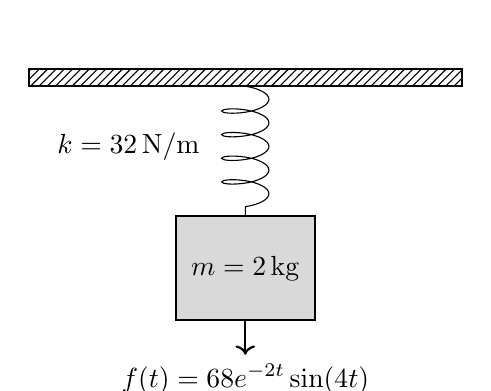
\begin{tikzpicture}[scale=1.1]
  % ceiling
  \draw[thick,pattern=north east lines] (-2.5,0) rectangle (2.5,0.2);
  \draw[thick] (-2.5,0) -- (2.5,0);
  % spring
  \draw[decoration={coil,aspect=0.3,segment length=3mm,amplitude=3mm},decorate] (0,0) -- (0,-1.5);
  \node at (-1.35,-0.7) {$k=32\,\mathrm{N/m}$};
  % mass
  \draw[fill=gray!30,thick] (-0.8,-1.5) rectangle (0.8,-2.7);
  \node at (0,-2.1) {$m=2\,\mathrm{kg}$};
  % forcing label and arrow
  \draw[->,thick] (0,-2.7) -- (0,-3.1);
  \node[below] at (0,-3.1) {$f(t)=68e^{-2t}\sin(4t)$};
\end{tikzpicture}%
}
\par\vspace{0.5em}\small\textit{Driven undamped mass--spring configuration}
\end{minipage}
\end{figure}

\subsection*{Solution}
\begin{stepbox}
\textbf{Stage 1: Set up the differential equation.}
\begin{enumerate}
  \item The equation of motion for an undamped spring-mass system with external forcing is \(m\,x'' + k\,x = f(t)\).
  \item Substitute \(m=2\) kg, \(k=32\) N/m, and \(f(t)=68e^{-2t}\sin(4t)\): \(2\,x'' + 32\,x = 68e^{-2t}\sin(4t)\).
  \item Divide by \(2\): \(x'' + 16x = 34e^{-2t}\sin(4t)\).
  \item Initial conditions: \(x(0) = 0\) (at equilibrium), \(x'(0) = 0\) (at rest).
\end{enumerate}
\end{stepbox}

\begin{stepbox}
\textbf{Stage 2: Solve the homogeneous equation.}
\begin{enumerate}
  \item Characteristic equation: \(r^2 + 16 = 0\) \(\Rightarrow\) \(r = \pm 4i\).
  \item Natural frequency: \(\omega_0 = 4\) rad/s.
  \item Homogeneous solution: \(x_h(t) = C_1\cos(4t) + C_2\sin(4t)\).
\end{enumerate}
\end{stepbox}

\begin{stepbox}
\textbf{Stage 3: Find particular solution by undetermined coefficients.}
\begin{enumerate}
  \item Try \(x_p(t) = e^{-2t}\big[A\cos(4t) + B\sin(4t)\big]\).
  \item Compute derivatives:
  \[
    x_p'(t) = e^{-2t}\big[(4B - 2A)\cos(4t) + (-4A - 2B)\sin(4t)\big],
  \]
  \[
    x_p''(t) = e^{-2t}\big[(-12A - 16B)\cos(4t) + (16A - 12B)\sin(4t)\big].
  \]
  \item Substitute into \(x_p'' + 16x_p = 34e^{-2t}\sin(4t)\) and simplify:
  \[
    e^{-2t}\big[(4A - 16B)\cos(4t) + (16A + 4B)\sin(4t)\big] = 34e^{-2t}\sin(4t).
  \]
  \item Match coefficients: \(4A - 16B = 0\) and \(16A + 4B = 34\).
  \item Solve: \(A = 4B\) and \(16(4B) + 4B = 34\) \(\Rightarrow\) \(B = \tfrac{1}{2}\), \(A = 2\).
  \item Particular solution: \(x_p(t) = e^{-2t}\left[2\cos(4t) + \tfrac{1}{2}\sin(4t)\right]\).
\end{enumerate}
\end{stepbox}

\begin{stepbox}
\textbf{Stage 4: Apply initial conditions.}
\begin{enumerate}
  \item General solution: \(x(t) = C_1\cos(4t) + C_2\sin(4t) + e^{-2t}\left[2\cos(4t) + \tfrac{1}{2}\sin(4t)\right]\).
  \item From \(x(0) = 0\): \(C_1 + 2 = 0\) \(\Rightarrow\) \(C_1 = -2\).
  \item Compute \(x'(t) = -4C_1\sin(4t) + 4C_2\cos(4t) + e^{-2t}\big[-9\sin(4t) - 2\cos(4t)\big]\).
  \item From \(x'(0) = 0\): \(4C_2 - 2 = 0\) \(\Rightarrow\) \(C_2 = \tfrac{1}{2}\).
\end{enumerate}
\end{stepbox}

\begin{stepbox}
\textbf{Final solution.}
\[
  \boxed{x(t) = -2\cos(4t) + \frac{1}{2}\sin(4t) + e^{-2t}\left[2\cos(4t) + \frac{1}{2}\sin(4t)\right].}
\]
The first term is the \emph{transient response} (decays as \(t\to\infty\)); the remaining terms form the \emph{steady-state response} (persists).
\end{stepbox}

\begin{codebox}
\begin{verbatim}
% verify_q9_correct.m
syms t
m = 2; k = 32;
A = 2; B = 1/2;
C1_val = -A;  % = -2
C2_val = (2*A - 4*B)/4;  % = 0.5

x_final = C1_val*cos(4*t) + C2_val*sin(4*t) + ...
          exp(-2*t)*(A*cos(4*t) + B*sin(4*t));

x_verify_prime = diff(x_final, t);
x_verify_double_prime = diff(x_verify_prime, t);

lhs = m*x_verify_double_prime + k*x_final;
rhs = 68*exp(-2*t)*sin(4*t);
ode_check = simplify(lhs - rhs);

assert(isequal(ode_check, sym(0)), 'ODE not satisfied!')
assert(abs(double(subs(x_final, t, 0))) < 1e-10, 'x(0) != 0')
assert(abs(double(subs(x_verify_prime, t, 0))) < 1e-10, 'x''(0) != 0')

fplot(x_final, [0, 8], 'LineWidth', 2);
grid on; xlabel('Time t (s)'); ylabel('Position x(t) (m)');
title('Driven Undamped Spring-Mass System');
exportgraphics(gcf, 'figures/q9_solution.png', 'Resolution', 300);
\end{verbatim}
\end{codebox}

\begin{resultsbox}
The solution is \(x(t) = -2\cos(4t) + \tfrac{1}{2}\sin(4t) + e^{-2t}\left[2\cos(4t) + \tfrac{1}{2}\sin(4t)\right]\). The forcing frequency \(4\) rad/s matches the natural frequency \(\omega_0 = 4\) rad/s, but the exponential decay prevents resonance. As \(t\to\infty\), the transient dies out and the system settles into a steady oscillation. The MATLAB verification confirms all conditions are satisfied. See Figure~\ref{fig:q9-solution}.
\end{resultsbox}

\begin{figure}[htbp]
\centering
\includegraphics[width=0.85\textwidth]{figures/q9_solution.png}
\caption{Position of the driven undamped spring-mass system. The transient response (green dashed) decays while the steady-state response (red dashed) persists. The total response (blue solid) is the sum of both.}
\label{fig:q9-solution}
\end{figure}

% ============================================================================
% Q10
% ============================================================================
\question{Question 10 (12 pts)}\label{quest:10}

The critical loads of thin columns depend on the end conditions of the column. Suppose we have a thin
vertical homogeneous column that is embedded at the base (\(x=0\)) and free at the top (\(x=L\)),
and that a constant axial load \(P\) is applied to the free end. The differential equation
for the deflection \(y(x)\) (for a small end displacement \(\delta\)) is
\[
EI\,\frac{d^2 y}{dx^2}+P\,y = P\,\delta.
\]
\begin{enumerate}
  \item What is the predicted \textbf{deflection} \(y(x)\) when \(\delta=0\)?
  \item When \(\delta\neq 0\), \textbf{show} that the Euler load for this column is \(P_h/4\),
  where \(P_h\) is the Euler load for a column hinged at both ends:
  \[
  P_h=\frac{\pi^2 E I}{L^2}.
  \]
\end{enumerate}

\begin{figure}[htbp]
\centering
\begin{minipage}{0.5\textwidth}
\centering
\fbox{%
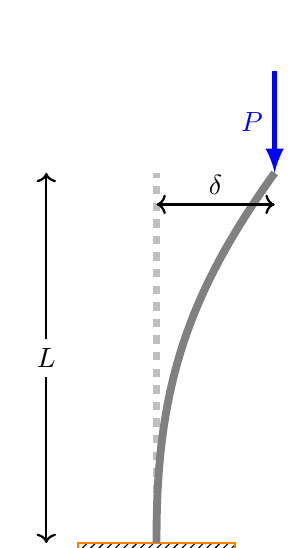
\begin{tikzpicture}[scale=1.0]
  % ground support
  \draw[pattern=north east lines, draw=orange, thick] (-1,0) rectangle (1,-0.2);
  % original column (dashed)
  \draw[line width=1mm, dashed, lightgray] (0,0) -- (0,4.7);
  % deflected shape
  \draw[line width=1mm, gray] (0,0) to[bend left=18] (1.5,4.7);
  % length dimension
  \draw[<->, thick] (-1.4,0) -- node[midway,fill=white] {$L$} (-1.4,4.7);
  % tip displacement
  \draw[<->, thick] (0,4.3) -- node[above] {$\delta$} (1.5,4.3);
  % applied load
  \draw[-latex, line width=.7mm, blue] (1.5,6) -- node[left] {$P$} (1.5,4.7);
\end{tikzpicture}%
}
\par\vspace{0.5em}\small\textit{Cantilever column under tip load}
\end{minipage}
\end{figure}

\subsection*{Solution}
\begin{stepbox}
\textbf{Part (a): Deflection when \(\delta = 0\).}
\begin{enumerate}
  \item When \(\delta = 0\), the ODE becomes: \(EI\,y'' + P\,y = 0\).
  \item Let \(\lambda^2 = P/EI\). Then: \(y'' + \lambda^2 y = 0\).
  \item General solution: \(y(x) = C_1\cos(\lambda x) + C_2\sin(\lambda x)\).
  \item Apply \(y(0) = 0\): \(C_1 = 0\).
  \item Apply \(y'(0) = 0\): \(C_2\lambda = 0\) \(\Rightarrow\) \(C_2 = 0\).
  \item This gives \(y(x) = 0\) (trivial solution).
\end{enumerate}
\[
  \boxed{\text{Answer (a): } y(x) = 0.}
\]
This makes physical sense: without lateral displacement, a perfectly straight column under axial load has no deflection (until buckling).
\end{stepbox}

\begin{stepbox}
\textbf{Part (b): Euler load when \(\delta \neq 0\).}
\begin{enumerate}
  \item ODE: \(y'' + \lambda^2 y = \lambda^2\delta\), where \(\lambda^2 = P/EI\).
  \item General solution: \(y(x) = C_1\cos(\lambda x) + C_2\sin(\lambda x) + \delta\).
  \item Apply \(y(0) = 0\): \(C_1 + \delta = 0\) \(\Rightarrow\) \(C_1 = -\delta\).
  \item Apply \(y'(0) = 0\): \(C_2\lambda = 0\) \(\Rightarrow\) \(C_2 = 0\).
  \item Solution: \(y(x) = \delta\big(1 - \cos(\lambda x)\big)\).
  \item Apply \(y''(L) = 0\) (zero moment at free end):
  \[
    y''(L) = \delta\lambda^2\cos(\lambda L) = 0.
  \]
  \item For nontrivial solution: \(\cos(\lambda L) = 0\) \(\Rightarrow\) \(\lambda L = \pi/2\) (smallest value).
  \item Therefore: \(\lambda = \pi/(2L)\).
  \item Since \(\lambda^2 = P/EI\):
  \[
    P = \lambda^2 EI = \frac{\pi^2 EI}{4L^2}.
  \]
  \item The hinged-hinged Euler load is \(P_h = \pi^2 EI/L^2\).
  \item Thus: \(P = \pi^2 EI/(4L^2) = P_h/4\).
\end{enumerate}
\[
  \boxed{\text{Answer (b): } P = \frac{P_h}{4} = \frac{\pi^2 EI}{4L^2}.}
\]
\end{stepbox}

\begin{codebox}
\begin{verbatim}
% solve_q10.m
syms x L P EI delta lambda real positive

% Part (a): delta = 0
% ODE: EI*y'' + P*y = 0
% Solution: y(x) = 0 (trivial)

% Part (b): delta ~= 0
% ODE: y'' + lambda^2*y = lambda^2*delta
% Solution: y(x) = delta*(1 - cos(lambda*x))
% Boundary condition y''(L) = 0 gives:
%   cos(lambda*L) = 0
%   lambda*L = pi/2
%   lambda = pi/(2*L)
%
% Critical load:
%   P = lambda^2*EI = pi^2*EI/(4*L^2)
%   P_h = pi^2*EI/L^2 (hinged-hinged)
%   P = P_h/4

% Verification
L_val = 1; EI_val = 1;
P_crit = pi^2*EI_val/(4*L_val^2);
P_h = pi^2*EI_val/L_val^2;
assert(abs(P_crit - P_h/4) < 1e-10, 'P ~= P_h/4');

disp('Verification passed: P = P_h/4');
\end{verbatim}
\end{codebox}

\begin{resultsbox}
\textbf{Part (a):} When \(\delta = 0\), the deflection is \(y(x) = 0\).

\textbf{Part (b):} The Euler critical load for the cantilever column is \(P = \pi^2EI/(4L^2) = P_h/4\), where \(P_h = \pi^2EI/L^2\) is the Euler load for a hinged-hinged column. The cantilever has one-quarter the critical load due to the fixed boundary at the base and free boundary at the top. The deflection shape is \(y(x) = \delta\big(1 - \cos(\pi x/(2L))\big)\). See Figure~\ref{fig:q10-solution}.
\end{resultsbox}

\begin{figure}[htbp]
\centering
\includegraphics[width=0.9\textwidth]{figures/q10_solution.png}
\caption{Left: Deflection shapes of the cantilever column for different load levels. Right: Comparison of critical loads showing \(P_{\text{crit}}/P_h = 1/4\).}
\label{fig:q10-solution}
\end{figure}

\subsection*{Additional Analysis: Comparison of All Column Types}

For a comprehensive understanding of Euler buckling, we compare all four standard boundary conditions. The critical load for each configuration is given by:
\[
  P_{\text{crit}} = \frac{\pi^2 EI}{(KL)^2} = \frac{\pi^2 EI}{L_{\text{eff}}^2},
\]
where \(K\) is the effective length factor and \(L_{\text{eff}} = KL\) is the effective buckling length.

\begin{table}[h]
\centering
\begin{tabular}{|l|c|c|c|}
\hline
\textbf{Boundary Condition} & \textbf{K Factor} & \textbf{\(L_{\text{eff}}\)} & \textbf{\(P_{\text{crit}}/P_h\)} \\
\hline
Fixed-Fixed (both ends clamped) & 0.5 & \(0.5L\) & 4.00 \\
Fixed-Pinned (one fixed, one pinned) & 0.699 & \(0.699L\) & 2.05 \\
Pinned-Pinned (both ends hinged) & 1.0 & \(1.0L\) & 1.00 \\
Fixed-Free (cantilever) & 2.0 & \(2.0L\) & 0.25 \\
\hline
\end{tabular}
\caption{Effective length factors and relative critical loads for different column boundary conditions. Reference: \(P_h = \pi^2EI/L^2\) (pinned-pinned).}
\label{tab:column-comparison}
\end{table}

\begin{figure}[htbp]
\centering
\includegraphics[width=0.95\textwidth]{figures/column_buckling_comparison.png}
\caption{Comprehensive comparison of Euler buckling for all standard boundary conditions. Left: Deflection shapes showing characteristic mode shapes. Top right: Relative critical loads normalized by pinned-pinned case. Bottom right: Effective length factors K.}
\label{fig:column-comparison}
\end{figure}

\begin{figure}[htbp]
\centering
\includegraphics[width=0.95\textwidth]{figures/column_boundary_conditions.png}
\caption{Side-by-side comparison of column buckling modes with boundary condition symbols. Fixed ends are shown as gray blocks, pinned ends as circles, and the free end with an applied load arrow. Each panel shows the deflected shape, K factor, and relative critical load.}
\label{fig:column-boundaries}
\end{figure}


\end{document}
